\documentclass[11pt]{article}
\usepackage[utf8]{inputenc}
\usepackage[T1]{fontenc}
\usepackage{amsmath}
\usepackage{amsfonts}
\usepackage{amssymb}
\usepackage[version=4]{mhchem}
\usepackage{stmaryrd}
\usepackage{graphicx}
\usepackage[export]{adjustbox}
\graphicspath{ {./images/} }

\begin{document}
Systematic Trading

Systematic trading is usually quantitative in nature and often referred to as computer-based, model-based, or black-box trading. Systematic trading in this context refers to the automation of the investment process, not to systematic risk. Systematic trading models apply a fixed set of trading rules in determining when to enter and exit positions. Deviation from the system's rules is generally not permitted.

\section*{Derivation of Systematic Trading Rules}
Systematic trading rules are generally derived from backtests. In the context of systematic trading rules, a backtest is an identification of a price or return pattern that appears to persist, as located and verified through a quantitative analysis of historical prices. Trading systems are generally based on the expectation that historical price patterns will recur in the future. However, many trading systems that appear to perform well using backtested data end up performing poorly when they are implemented in real time. Statistics show that when many analysts search through many data sets with many hypothetical trading systems, very many trading systems appear ex post to be profitable but in fact are generated purely by randomness or by market regimes that no longer exist. Being able to avoid data dredging and false identification of attractive trading rules is the key to successful backtesting.

Backtests should also have reasonable estimates for transaction costs and slippage. Slippage is the unfavorable difference between assumed entry and exit prices and the entry and exit prices experienced in practice. Thus, an analyst observing a long history of daily closing prices should assume that an actual trading strategy is likely to generate less favorable price executions due to the tendency of buy orders to push prices up, or be executed at an offer price, and of sell orders to push prices down, or be executed at a bid price. Care should also be taken to ensure that reported prices on which backtests are performed are executable prices rather than stale prices or published indications of prices, and that they are free from large errors. Systematic traders rarely employ only a single trading system with a single security.

Managers who have success with one trading system in one market typically search for other markets in which that trading system, or a modified version of it, can be successfully applied. Over time, managers may modify their trading systems, develop new ones, and abandon others.

\section*{Three Questions in Evaluating a Systematic Trading System}
There are three useful questions to ask when evaluating an individual trading strategy:

\begin{enumerate}
  \item What is the trading system, and how was it developed? Here, one is looking to understand the broad underlying trading approach (e.g., trend following versus countertrend) and specific characteristics of the strategy itself. It is also important to understand the research methods used to identify and develop the trading strategy to avoid strategies based on spurious results from data dredging. Poor research methods can lead to overfitting of historical data, such that a historical price series may appear to have a recurring pattern yet be in fact random.

  \item Why and when does the trading system work, and why and when might it not work? It is important to understand the underlying hypothesis of a specific trading strategy. If the trading system is making money for its investors, from where or from whom is that money coming? Such understanding is important in and of itself but is also critical in identifying market conditions that are likely to be supportive of the strategy (e.g., trend accompanied by low volatility). Although it may be difficult to forecast market conditions, understanding what impact various market conditions are likely to have on the strategy's performance is important in interpreting the potential success or failure of a strategy over time.

  \item How is the trading system implemented? Many operational factors contribute to a successful systematic trading strategy, including selection of data sources, determination of periodicity of data, establishment of protocols to clean the data, processing of the data into a trading signal, placement of trades, record keeping, and broker reconciliation.

\end{enumerate}

The key to systematic trading systems is to differentiate spurious results from results that will persist. Similarly, analysts seek to ascertain whether trading systems that were successful in the past but have stopped working recently will perform poorly on a temporary basis or on a permanent basis. In other words, at what point should a trading system be abandoned or modified if the system worked very well in the past but has generated poor results recently?

\section*{Validation and Potential Degradation of Systematic Trading Rules}
Systematic managed futures strategies rely on quantitative research methods that backtest trading rules using historical price data. Validation of a trading rule refers to the use of new data or new methodologies to test a trading rule developed on another set of data or with another methodology. For example, a trading rule developed analyzing data during five calendar years should be tested first in subperiods of those five years to see if the results are robust across data sets and subintervals. Robustness refers to the reliability with which a model or system developed for a particular application or with a particular data set can be successfully extended into other applications or data sets. Most important, validation of the trading rule should be performed with out-of-sample data. Out-of-sample data are observations that were not directly used to develop a trading rule or even indirectly used as a basis for knowledge in the research. For example, the trading rule should be validated on the most recent data, which, of course, should not have been used explicitly or implicitly in the model's development. In-sample data are those observations directly used in the backtesting process. Out-of-sample data consist of more recent data than were used in the backtest. Out-of-sample data should be used to test the profitability of a trading strategy beyond the period covered by the backtest. The goal is to avoid data dredging and to ensure that a trading rule generates persistent performance.

Further, it is vital to know how many trading rules were tested, how many were subjected to validation, and how many were rejected in the validation process. If 20 trading rules (e.g., one model with 20 different parameter values) are subjected to validation, one of them on average will survive a validation process with a confidence interval of $95 \%$, even if none of the rules truly offers value-added properties. More to the point, if several analysts test hundreds of strategies (e.g., hundreds of parameter values) on numerous data sets (e.g., securities), then numerous trading strategies will survive the validation process unless the validation process is carefully designed to incorporate into its statistical approach the total number of tests performed.

Trading rules typically evolve over time as analysts try to optimize profitability. Analysts perform ongoing research to estimate and refine trading parameters, add new trading parameters, and drop old trading parameters. Markets also typically evolve over time. A once-profitable price pattern that becomes identified and exploited by numerous CTAs eventually ceases to exist or substantially changes. Therefore, a trading model or trading strategy that has been successful over the past

10 years often experiences degradation and is not profitable over the next 10 years. In this context, degradation is the tendency and process through time by which a trading rule or trading system declines in effectiveness. The key is to differentiate between (1) trading rules that are being changed to better identify true price patterns, and (2) trading rules that are data dredging for a pattern that no longer exists. Both an effective trading system and a fully degraded trading system experience episodes of high returns and episodes of poor returns due to randomness. Identifying which systems remain effective and which have degraded requires careful statistical analysis as well as informed qualitative analysis.

\section*{Systematic Trading Strategies Overview}
Systematic trading strategies are generally categorized into three groups: trend-following, non-trend-following, and relative value.

Trend-following strategies are designed to identify and take advantage of momentum in price direction (i.e., trends in prices). Momentum is the extent to which a movement in a security price tends to be followed by subsequent movements of the same security price in the same direction. Trend-following strategies use recent price moves over some specific time period (e.g., ranging from a few minutes to several hundred days) to identify a price trend. The goal is to establish long positions in assets experiencing an upward trend, establish short positions in assets experiencing a downward trend, and avoid positions in assets not experiencing a trend.

Mean-reverting refers to the situation in which returns show negative autocorrelation-the opposite tendency of momentum or trending. An asset that consistently tends to return toward its previous price level after a move in one direction is typically said to be mean-reverting or to exhibit mean reversion. Mean reversion is the extent to which an asset's price moves toward the average of its recent price levels. Trending markets exhibit returns with positive autocorrelation. A price series with changes in its prices that are independent from current and past prices is a random walk. Therefore, momentum and mean reversion are properties that are not consistently displayed by prices that follow a random walk.

\section*{Simple Moving Averages in Systematic Trading Strategies}
One of the most popular classes of trend-following strategies uses moving averages to signal trades. A moving average is a series of averages that is recalculated through time based on a window of observations. The most basic approach uses a simple moving average, a simple arithmetic average of previous prices. More sophisticated averaging techniques place a greater weight on more recent prices. The formula for calculating a simple moving average, $S M A_{t}(n)$, is shown in Equation 1 , where $t$ is the current time period and $n$ is the number of time periods used in the computation:


\begin{equation*}
S M A_{t}(n)=\frac{1}{n} p_{t-1}+\frac{1}{n} p_{t-2}+\cdots+\frac{1}{n} p_{t-n} \tag{1}
\end{equation*}


The window of observations is composed of a fixed number of lagged prices. For example, a current 10-day moving average price (day 0 ) is formed using the 10 prices corresponding to the 10 days immediately preceding the current price (days -1 to -10 ). Yesterday's (day -1 ) 10-day moving average would be composed of the prices corresponding to the 10 days prior to that day (days -2 to -11 ). The next exhibit, Simple Moving Average Summary summarizes the process along with the classic trading signals based on a simple trend following rule.

Simple Moving Average Summary

Description: In a simple moving average, the daily prices are equally weighted. As each new price observation is added to the series, the oldest observation falls away, creating a window of averaged prices that is often charted.

Signals: $\quad$ Enter long if current price $P_{t}>S M A_{t}(n)$

Enter short if current price $P_{t}<S M A_{t}(n)$

Like the underlying market itself, the moving average price changes every day, but the moving average changes value in a lagged and muted fashion relative to the current price. The shorter the time period used to calculate the moving average, the more quickly the average will respond to changes in the level of more current prices, the more volatile the average will be, and, generally, the more times the current price will cross over the moving average price (i.e., the more trading signals will be generated).

Numerous variations of moving average computations exist:

\begin{itemize}
  \item The number of periods (and the length of the time period) used in the moving average, $n$, can vary (e.g., 10-day versus 30-day versus 60-minute).
  \item The entry and exit levels can be a percentage of the moving average (e.g., enter when the current price exceeds the moving average by $1 \%$ ).
  \item An unequally weighted moving average can be calculated, using an averaging process that weights recent prices more heavily than older prices.
\end{itemize}

There are trading signals other than the comparison of the current price to a single moving average. For example, trading signals to establish long positions may be identified as follows:

\begin{itemize}
  \item When the current price exceeds two or more moving averages (e.g., both the 10-day and the 30-day moving averages)
  \item When a shorter-term moving average crosses up and over a longer-term moving average
  \item When moving averages align upward (i.e., are all in the same direction, with the shorter moving averages exceeding the longer moving averages)
\end{itemize}

The three computational variations taken together with the various signal identification rules generate an astounding number of possible strategies. The abundance of potential strategies leads to the potential problem of data dredging, in which so many potential strategies can be tested that strategies will be identified that satisfy empirical tests with high levels of statistical confidence even when true patterns do not exist. There are two major approaches to weighting more recent prices more heavily than older prices: weighted moving averages and exponential moving averages.

\section*{Weighted and Exponential Moving Averages in Systematic Trading Strategies}
Although simple moving averages are the most commonly used measures, weighted and exponential moving averages are also used and have the potential advantage of assigning larger weights to the most recent prices.

A weighted moving average is usually formed as an unequal average, with weights arithmetically declining from most recent to most distant prices. To illustrate, the length of the averaging interval (i.e., the number of observations used in the computation of each average) is denoted as $n$. The oldest price is multiplied by 1 , the second oldest price is multiplied by 2 , and so forth, until the most recent price is multiplied by $n$. Each product is then divided by the sum of the digits. The $n$-period weighted moving average, $W M A_{t}(n)$, is shown in Equation 2:


\begin{align*}
& \text { Define } N=1+2+3+\cdots+n \\
& W M A_{t}(n)=\frac{n}{N} p_{t-1}+\frac{n-1}{N} p_{t-2}+\cdots+\frac{1}{N} p_{t-n} \tag{2}
\end{align*}


In the case of $n=4$, the sum of the labels, $N$, is 10 (the sum of 1 through 4). The most recent previous price $\left(P_{t-1}\right)$ is weighted $40 \%(4 / 10)$, the second most recent price is weighted $30 \%(3 / 10)$, and so forth, until the oldest price is weighted only $10 \%(1 / 10)$. Note that the weights decline arithmetically: $40 \%, 30 \%, 20 \%$, and $10 \%$.

The exponential moving average is a geometrically declining moving average based on a weighted parameter, $\lambda$, with $0<\lambda<1$. The most recent observation is weighted through multiplication by the weighted parameter, $\lambda$. All other previous observations are weighted by $\lambda(1-\lambda)^{n}$, in which $n$ is the length of the time lag. For example, with $\lambda=0.4$, the most recent observation is multiplied by 0.4 . The second and third most recent observations are weighted by $\lambda(1-\lambda)^{1}$ and $\lambda(1-\lambda)^{2}(0.24$ and 0.144), respectively. The formula for the exponential moving average at time $t, E M A_{t}(\lambda)$, is given next in an expanded form (Equation 3a) and a reduced form (Equation 3b):

$$
\begin{gathered}
E M A_{t}(\lambda)=\lambda P_{t-1}+\lambda(1-\lambda) P_{t-2}+\lambda(1-\lambda)^{2} P_{t-3}+\lambda(1-\lambda)^{3} P_{t-4}+\cdots \\
E M A_{t}(\lambda)=\left(\lambda \times P_{t-1}\right)+\left[(1-\lambda) \times E M A_{t-1}(\lambda)\right]
\end{gathered}
$$

Equation 3a illustrates the intuition of the exponential moving average. The most recent price receives the weighted parameter, $\lambda$. The terms after the first term are multiplied both by $\lambda$ and by $(1-\lambda)^{n}$. Since $(1-\lambda)$ is less than 1 , the weight assigned to each previous price declines as the price becomes more distant. The problem with Equation 3a is that to compute $E M A_{t}(\lambda)$ using that equation requires input of the entire history of the price series.

Equation 3b denotes how the exponential moving average is calculated in practice. In this view, today's exponential moving average is a weighted average of the current price and yesterday's exponential moving average. Inspection of either equation reveals that the formula requires an infinitely long history of previous prices. Therefore, in practice, computation is performed by seeding some initial value to $E M A_{t-1}$. Once an initial approximation is set for a previous value of the exponential moving average, all subsequent exponential moving averages are simply computed as the sum of $\lambda$ times the most recent price $(1-\lambda)$ times the most recent exponential moving average.

\section*{An Illustration of a System Using Two Moving Averages}
The next exhibit illustrates a strategy employing two moving averages to generate trading signals. In the example, the strategy uses a 10-day and a 45-day moving average as the shorter-term and the longer-term indicators, respectively. The first signal in the example (denoted with a vertical line) is a sell signal (i.e., a signal to establish a short position), because the 10-day moving average line (the shorter average) crossed below the 45-day moving average line (the longer average). Some days later, a signal to establish a long position emerged when the 10-day moving average line crossed above the 45-day moving average line.

\section*{10-Day and 45-Day SMA with Price Data}
\begin{center}
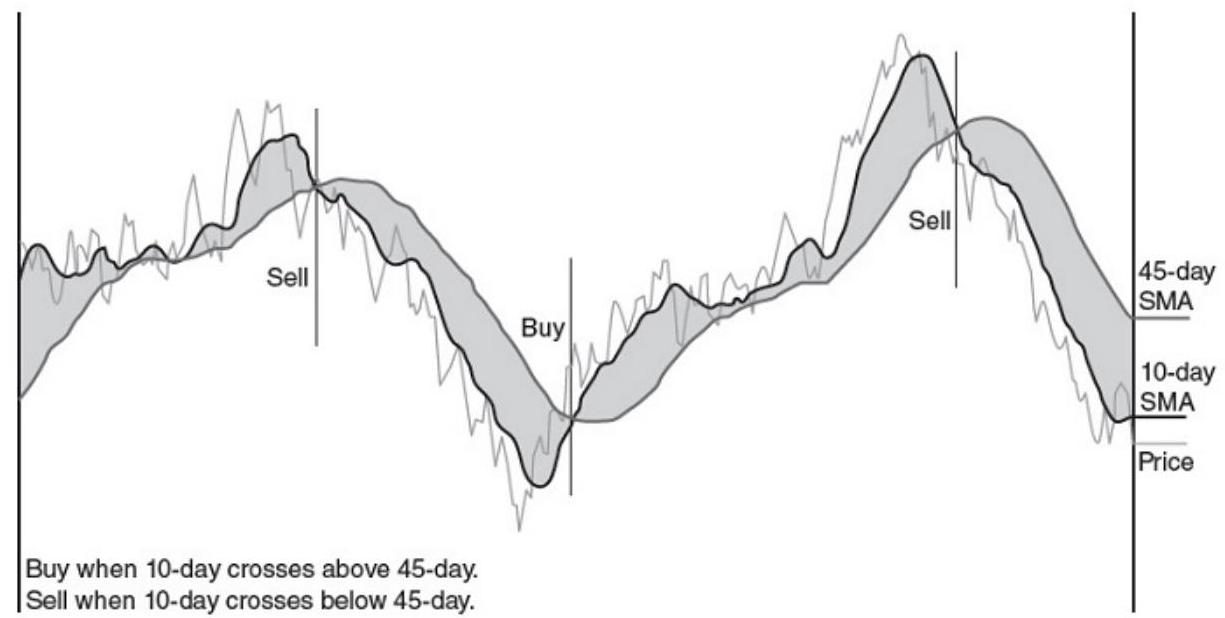
\includegraphics[max width=\textwidth]{2024_04_09_5d84553069220c8df1d0g-05}
\end{center}

\section*{Example with Two Moving Averages}
Example with Two Moving Averages appears to illustrate a highly successful trading period with two sell signals at prices much higher than the buy signal. Trendfollowing strategies perform well when there is an extended move in the price from one level to another, and tend to be more powerful when that move is accompanied by low daily price volatility. This low volatility makes it less likely that the trend-following manager will be whipsawed. Whipsawing is when a trader alternates between establishing long positions immediately before price declines and establishing short positions immediately before price increases and, in so doing, experiences a sequence of losses. In trend-following strategies, whipsawing results from a sideways market. A sideways market exhibits volatility without a persistent direction. The above exhibit contains several regions in which whipsawing may take place. Midway between the starting point and the first indicated trade signal are two instances where the two moving averages appear to touch and then return to their previous relationship. When trading signals are clustered, whipsawing generally takes place, and traders lose from the accompanying back-and-forth price pattern as well as the trading costs (bid-ask spreads and commissions).

Visual exhibits with discrete prices tend to mask the potential for whipsawing and its trading costs. Also, when a market price consistently reverts toward previous values (i.e., is mean-reverting), trend-following strategies tend to generate negative alphas. The primary challenge of implementing a moving average strategy is forecasting when markets are likely to trend, meaning the strategy should be applied, and forecasting when markets are likely to be random or to mean-revert, meaning the strategy should not be applied. Thus, implementation of moving average strategies focuses on developing methods of determining when to apply the strategy in addition to specifying which particular moving average strategy to apply. There has been considerable academic debate over the viability of trendfollowing strategies.

\section*{Breakout Strategies}
Breakout strategies focus on identifying the commencement of a new trend by observing the range of recent market prices (e.g., looking back at the range of prices over a specific time period). If the current price is below all prices in the range, the strategy identifies this as a breakout and possibly the beginning of a downward trend, and a short position is initiated. Breakout strategies lead to long trade entry points when prices break above these ranges. If a price is within the range, then the system might continue to hold the previous position or no position at all. The concept can apply to both prices and volatilities, and these are often used in tandem. Channel Breakout Strategy Summary describes a simple channel breakout strategy.

The simplest way to think of this is in terms of a look-back. For example, a 20-day look-back means that the trading system observes today's price in relation to all prices over the past 20 days. The next exhibit provides a summary.

Channel Breakout Strategy Summary

\begin{center}
\begin{tabular}{|ll|}
\hline
Description: & Channels are created by plotting the range of new price highs and lows. When one side grows disproportionately to the other, a trend is revealed. \\
Signals: & Buy when channel breaks upward;  Sell when channel breaks downward. \\
Equation: & UpperBound $=$ HighestHigh $(n)$ ; LowerBound $=$ LowestLow $(n)$ ; Most commonly, $n=20$ days \\
\end{tabular}
\end{center}

\section*{Analysis of Trend-Following Strategies}
Trend following is generally believed to be the dominant strategy applied in managed futures, in terms of both numbers of managers and the amount of industry assets. Empirical analysis by Fung and Hsieh confirms that trend following is the dominant style employed by CTAs. ${ }^{1}$ William Fung and David Hsieh, "Empirical Characteristics of Dynamic Trading Strategies: The Case of Hedge Funds," Review of Financial Studies 10, no. 2 (April 1997): 275-302.

Lhabitant explains two drawbacks of trend-following systems based on moving average rules. ${ }^{2}$ FranÇois-Serge Lhabitant, Hedge Funds: Origine, Strategies, Performance (Paris: Dunod, 2008). First, they are slow to recognize the beginning or end of trends. That is, an entry signal occurs after the trend has already been in effect for a while and profits have been missed, and the exit signal occurs after the trend has reversed and losses have occurred. The second drawback is that moving average rules are designed to exploit trends or momentum that should not persist in competitive markets. Perfect competition causes randomness rather than trending in price. But even at modest levels of competition, trends may cease to exist at approximately the same time that they become easily identified. In this case, moving average rules tend to generate useless and costly signals; that is, the trader may end up incurring substantial transaction costs and being whipsawed.

Some observers have described trend-following strategies as long volatility strategies. The idea is that trend-following strategies profit when market prices make large unidirectional changes and that large unidirectional changes generate higher reported volatility, as indicated by some measures of volatility. However, large unidirectional changes can also be consistent with low volatility. For example, a prolonged period of consistently positive daily or weekly returns compounds into large monthly returns and a large unidirectional change. But the standard deviation of the daily or weekly returns will be low if most of the returns are near the mean return. Thus, depending on how volatility is viewed or measured, trend-following systems may or may not be accurately described as being long volatility.

Malek and Dobrovolsky provide an extended discussion of the volatility exposure of managed futures programs. ${ }^{3}$ Marc H. Malek and Sergei Dobrovolsky, "Volatility Exposure of CTA Programs and Other Hedge Fund Strategies," Journal of Alternative Investments 11, no. 4 (2009): 68-89. Rather than describing CTAs as managers who take long volatility positions, Malek and Dobrovolsky assert that a better view is that CTAs take long gamma positions. Gamma is more completely discussed in the session, Event-Driven and Relative Value Hedge Funds. In this context, gamma refers to the risk exposure from increasing long positions in rising markets and decreasing short positions in falling markets.

Managed futures programs can benefit when markets trade in wide ranges, making prolonged moves between levels that vary substantially. Trend-following programs struggle to profit when markets trade in narrow ranges and exhibit negative autocorrelation. Predicting those markets that will consistently experience trends, and identifying when those markets are going to trend-and when they will not trend-is the goal of many CTAs and the source of alpha.

\section*{Non-Trend-Following Strategies}
Non-trend-following strategies are designed to exploit nonrandomness in market movements, such as a pattern of relative moves in prices of related commodities (e.g., oil and gasoline). Non-trend-following strategies generally fall into the major categories of countertrend or pattern recognition. Countertrend strategies use various statistical measures, such as price oscillation or a relative strength index, to identify range-trading opportunities rather than price-trending opportunities. The relative strength index (RSI), sometimes called the relative strength indicator, is a signal that examines average up and down price changes and is designed to identify trading signals such as the price level at which a trend reverses (See next exhibit, Relative Strength Index (RSI)). The formula for RSI is shown in Equation 4.


\begin{equation*}
R S I=100-\frac{100}{1+\frac{U}{D}} \tag{4}
\end{equation*}


where $U=$ average of all price changes for each period with positive price changes for the last $n$ periods, $D=$ average of all price changes (expressed as absolute values) for each period with negative price changes for the last $n$ periods, and $n=$ number of periods (most commonly, $n=14$ days).

Relative Strength Index (RSI)

Description: The RSI is an oscillator based on an index of 0 (a market low) to 100 (a market high), with 50 being neutral. The RSI attempts to determine the relative market strength of the current price. To do this, the RSI compares the average price change for each period having a positive price change with the average price change for each period having a negative price change.

Signals: $\quad$ Establish long position when RSI $<30$ (oversold market).\\
Signals: $\quad$ Establish short position when RSI $> 70$ (overbought market).

An example of applying the RSI is summarized in the next exhibit, Relative Strength Index (RSI); Sometimes Termed Relative Strength Indicator. The RSI is a simple form of a pattern recognition system. A pattern recognition system looks to capture non-trend-based predictable abnormal market behavior in prices or volatilities. The RSI can be implemented with any periodicity or unit of time. The periodicity, $N$, is defined as days, and the number of periods is often set at 14 days. But the periodicity can be expressed in hours, in minutes, or even in terms of individual price ticks; the user sets the number of periods.

\begin{center}
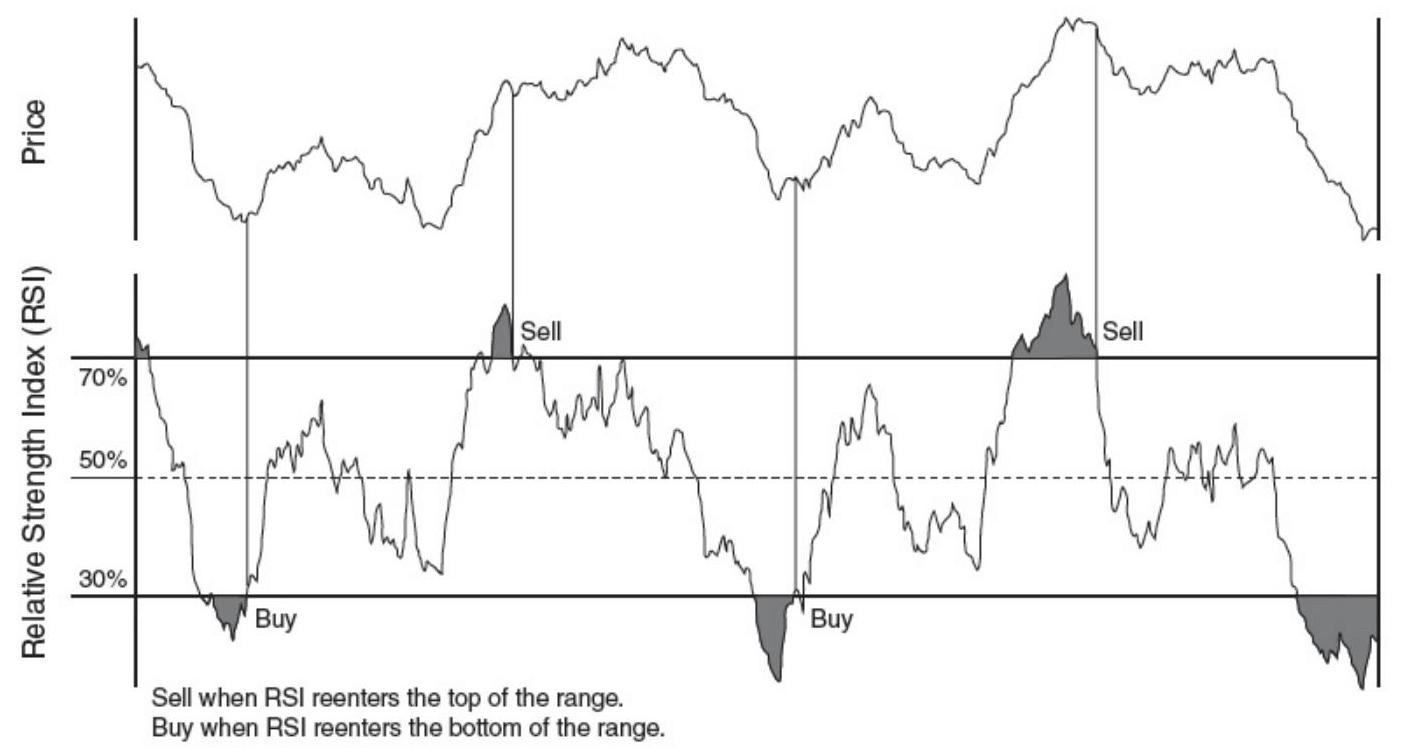
\includegraphics[max width=\textwidth]{2024_04_09_5d84553069220c8df1d0g-07}
\end{center}

Relative Strength Index (RSI); Sometimes Termed Relative Strength Indicator

The RSI trading signals are based on numerical levels. When an RSI is less than 30, the market is typically considered oversold (i.e., underpriced), and a long position is established. When its value is more than 70, the market is considered overbought, and a short position is taken. Relative Strength Index (RSI); Sometimes Termed Relative Strength Indicator illustrates the use of an RSI graphically using hypothetical data. As can be seen in the diagram, the price of a futures contract declined sharply early in the series, eventually reaching a level for which the corresponding RSI was less than 30, indicated by the dark-shaded area below the $30 \%$ RSI horizontal line. At or below this level, the countertrend strategy would buy (i.e., go long) the futures contract and hold the position (subject to other risk management rules in the strategy) until the RSI moved back into its midrange, where it might be liquidated. As prices continued to move higher, so did the RSI, eventually reaching levels associated with an overbought market. The strategy would then signal the trader to establish a short futures position, once again hoping to liquidate the position when the RSI returned to its midrange.

Relative strength index applications vary in terms of the timing of transactions. For example, a buy or entering trade might be made when the RSI reaches 30 from above, when it returns to 30 from below, or even using more sophisticated analysis to select a point while the RSI is below 30 . The above exhibit illustrates basing buy decisions on when the RSI reaches 30 from below and sell decisions when the RSI reaches 70 from above.

The above exhibit portrays a very successful example of using the RSI. Prolonged downtrends and uptrends can generate losses. Non-trend-following strategies trade frequently, usually much more often than do most trend-following systems, although short-term trend-following strategies are likely to have high turnover as well. In the managed futures industry, most countertrend strategies operate within a relatively short time frame, using periods ranging from minutes to a few days. This higher frequency price sampling, at least relative to trend followers, more often than not results in substantially higher daily trading volumes. For instance, many trend followers trade between 1,000 and 2,000 contracts annually per $\$ 1$ million AUM, whereas nontrend managers frequently trade 5,000 or more contracts per $\$ 1$ million AUM.

\section*{Relative Value Strategies and Technical Analysis}
Relative value strategies attempt to capture inefficient short-term price divergences between two empirically or theoretically correlated prices or rates. Technical strategies commonly applied to prices and rates can also be applied to spreads or ratios between prices and rates in relative value strategies. For example, RSIs can be applied to the price spread between related assets, such as the spread between the futures price of corn and the futures price of wheat.

In managed futures, relative value strategies focus on short time frames (e.g., measured in seconds to days) or long time frames (e.g., measured in months). Relative value strategies analyze the correlation structure between two or more futures contracts and attempt to exploit deviations in prices as individual futures contracts respond differently to new information or to liquidity imbalances.

The next exhibit illustrates a relative value futures trade. It depicts the price evolution of two contracts, A and B, which are assumed to be highly correlated (e.g., oil and gasoline). Assume that earlier in the series, prior to the time period graphed in the next exhibit, the prices of both contracts behaved very similarly. However, as illustrated in the exhibit below, after reaching an initial low, the price of contract A rose much faster than the price of contract B. Relative value strategies look to exploit the price gap that developed between these two contracts by selling (i.e., going short) contract A and buying (i.e., going long) contract B when the spread becomes large relative to past spreads. The trade is unwound as the two price series converge.

\begin{center}
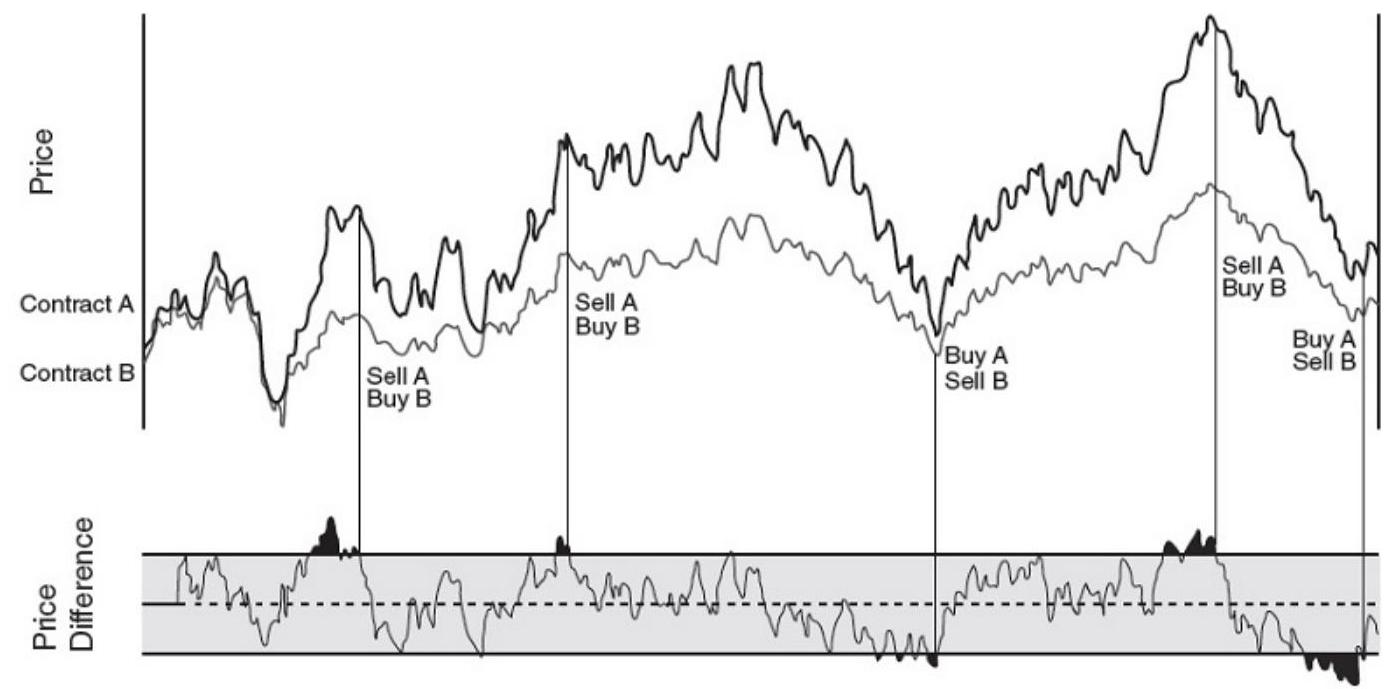
\includegraphics[max width=\textwidth]{2024_04_09_5d84553069220c8df1d0g-08}
\end{center}

Trade the spread when the relationship of the instruments is unbalanced.

\section*{Relative Value Strategy}
The relative value strategy does not directly rely on the separate behavior of either price series. In other words, it is not essential that price A or price B experience trending or mean reversion. Rather, the focus is on the behavior of the relationship between the two prices.

The strategies outlined here are just a few of those used in managed futures trading. In practice, these trading strategies are often quite complex, containing a variety of rules and filters, entries, exits, position sizing, and risk management.


\end{document}